\begin{tikzpicture}[
    >=Latex,
    font=\small,
    scale=0.55
]

%%%%%%%%%%%%%%%%%%%%%%%%%%%%%%%%%%%%%%%%%%%%%%
% Plane H_G
%%%%%%%%%%%%%%%%%%%%%%%%%%%%%%%%%%%%%%%%%%%%%%

\coordinate (A) at (-7,-2);
\coordinate (B) at ( 5,-2);
\coordinate (C) at ( 8, 0.6);
\coordinate (D) at (-4, 0.6);

\filldraw[
    fill=red!6,
    draw=red!60,
    line width=.6pt
]
(A)--(B)--(C)--(D)--cycle;

\node[
     red!85!black,
    font=\Large\itshape
]
at (7.4,-1.6)
{$H_G$};

\node[
     red!85!black,
    font=\Large\itshape
]
at (-5.4,-1.4)
{$\eta$};

%%%%%%%%%%%%%%%%%%%%%%%%%%%%%%%%%%%%%%%%%%%%%%
% Symmetric states
%%%%%%%%%%%%%%%%%%%%%%%%%%%%%%%%%%%%%%%%%%%%%%

\coordinate (S1) at (-3.8,-0.3);
\coordinate (S2) at ( 3.8,-1);

\fill[red] (S1) circle (2.8pt);
\fill[red] (S2) circle (2.8pt);

%%%%%%%%%%%%%%%%%%%%%%%%%%%%%%%%%%%%%%%%%%%%%%
% Non-symmetric state
%%%%%%%%%%%%%%%%%%%%%%%%%%%%%%%%%%%%%%%%%%%%%%

% Same x-coordinate as S1:
\coordinate (N) at (-3.8,3.3);

\fill[gray!70] (N) circle (2.8pt);

%%%%%%%%%%%%%%%%%%%%%%%%%%%%%%%%%%%%%%%%%%%%%%
% Projection / symmetrization arrow
%%%%%%%%%%%%%%%%%%%%%%%%%%%%%%%%%%%%%%%%%%%%%%

\draw[
    dashed,
    gray!70,
    line width=0.8pt,
    -{Latex[length=2.5mm]}
]
(N) -- (S1);

\node[
    gray,
    font=\itshape,
    align=center
]
at (-2.2,1.5)
{Section \ref{sec:symmetrization-of-the-variational-posterior}};

%%%%%%%%%%%%%%%%%%%%%%%%%%%%%%%%%%%%%%%%%%%%%%
% Red path in H_G
%%%%%%%%%%%%%%%%%%%%%%%%%%%%%%%%%%%%%%%%%%%%%%

\draw[
    red!85!black,
    line width=2pt
]
(S1)
.. controls (-1.5,0.15)
        and ( 1.5,-0.55)
..
(S2);

%%%%%%%%%%%%%%%%%%%%%%%%%%%%%%%%%%%%%%%%%%%%%%
% Direction arrow on path
%%%%%%%%%%%%%%%%%%%%%%%%%%%%%%%%%%%%%%%%%%%%%%

\draw[
    red!85!black,
    line width=1.5pt,
    -{Latex[length=3mm]}
]
(0.65,-0.42) -- (0.95,-0.44);

%%%%%%%%%%%%%%%%%%%%%%%%%%%%%%%%%%%%%%%%%%%%%%
% Labels
%%%%%%%%%%%%%%%%%%%%%%%%%%%%%%%%%%%%%%%%%%%%%%

\node[
    left
]
at ($(S1)+(-0.2,0.5)$)
{};

\node[
    right
]
at ($(S2)+(0.2,0.4)$)
{};

\node[
    below=4mm
]
at (N)
{\Large};

\node[
    red!75!black,
    font=\itshape
]
at (1.1,0.15)
{Theorem \ref{thm:equivariance-of-vi}};

%%%%%%%%%%%%%%%%%%%%%%%%%%%%%%%%%%%%%%%%%%%%%%
% Left inset
%%%%%%%%%%%%%%%%%%%%%%%%%%%%%%%%%%%%%%%%%%%%%%

\node[
    draw=red!35,
    rounded corners=2pt,
    fill=white,
    inner sep=2pt
]
(PlotL)
at (-7,1.0)
{
    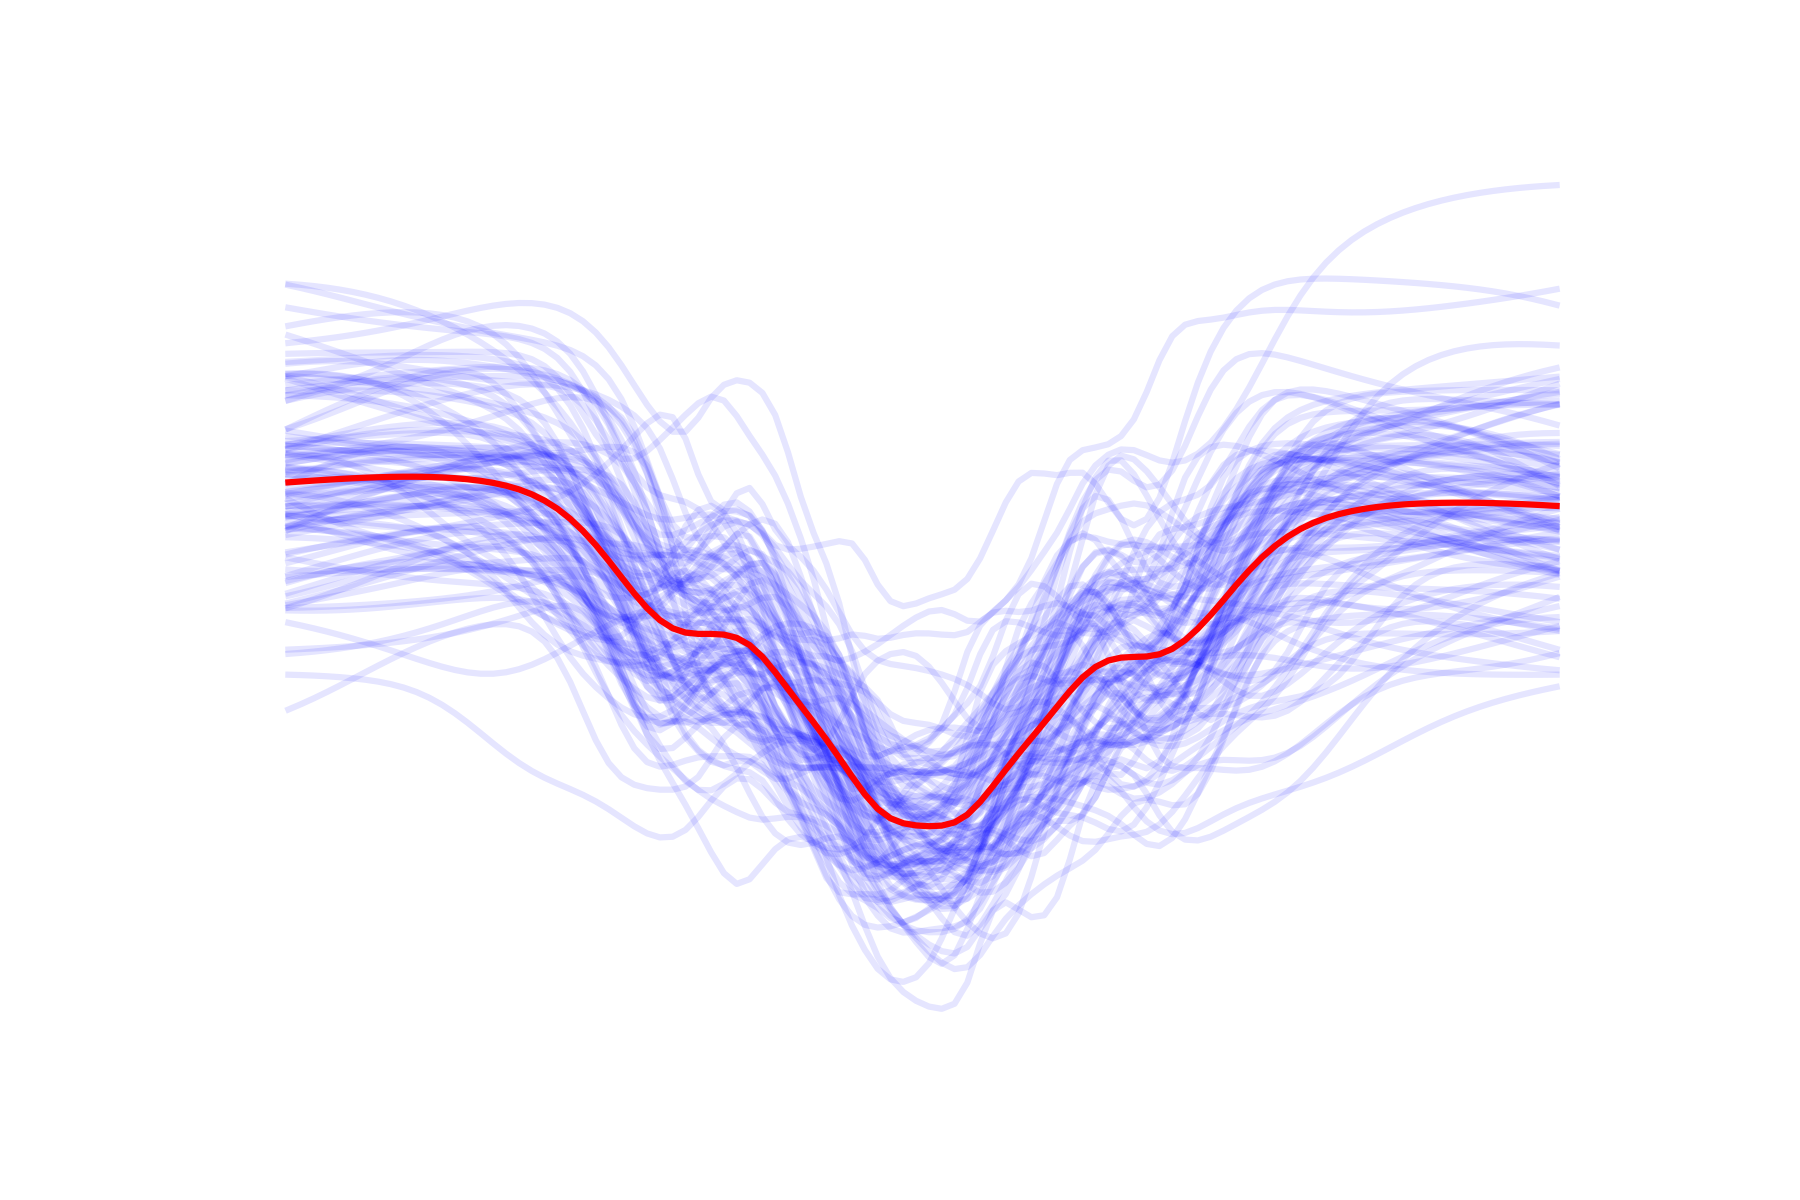
\includegraphics[width=1.8cm]{symnet_2.png}
};



%%%%%%%%%%%%%%%%%%%%%%%%%%%%%%%%%%%%%%%%%%%%%%
% Top inset
%%%%%%%%%%%%%%%%%%%%%%%%%%%%%%%%%%%%%%%%%%%%%%

\node[
    draw=black!35,
    rounded corners=2pt,
    fill=white,
    inner sep=2pt
]
(PlotN)
at (-1,3.3)
{
    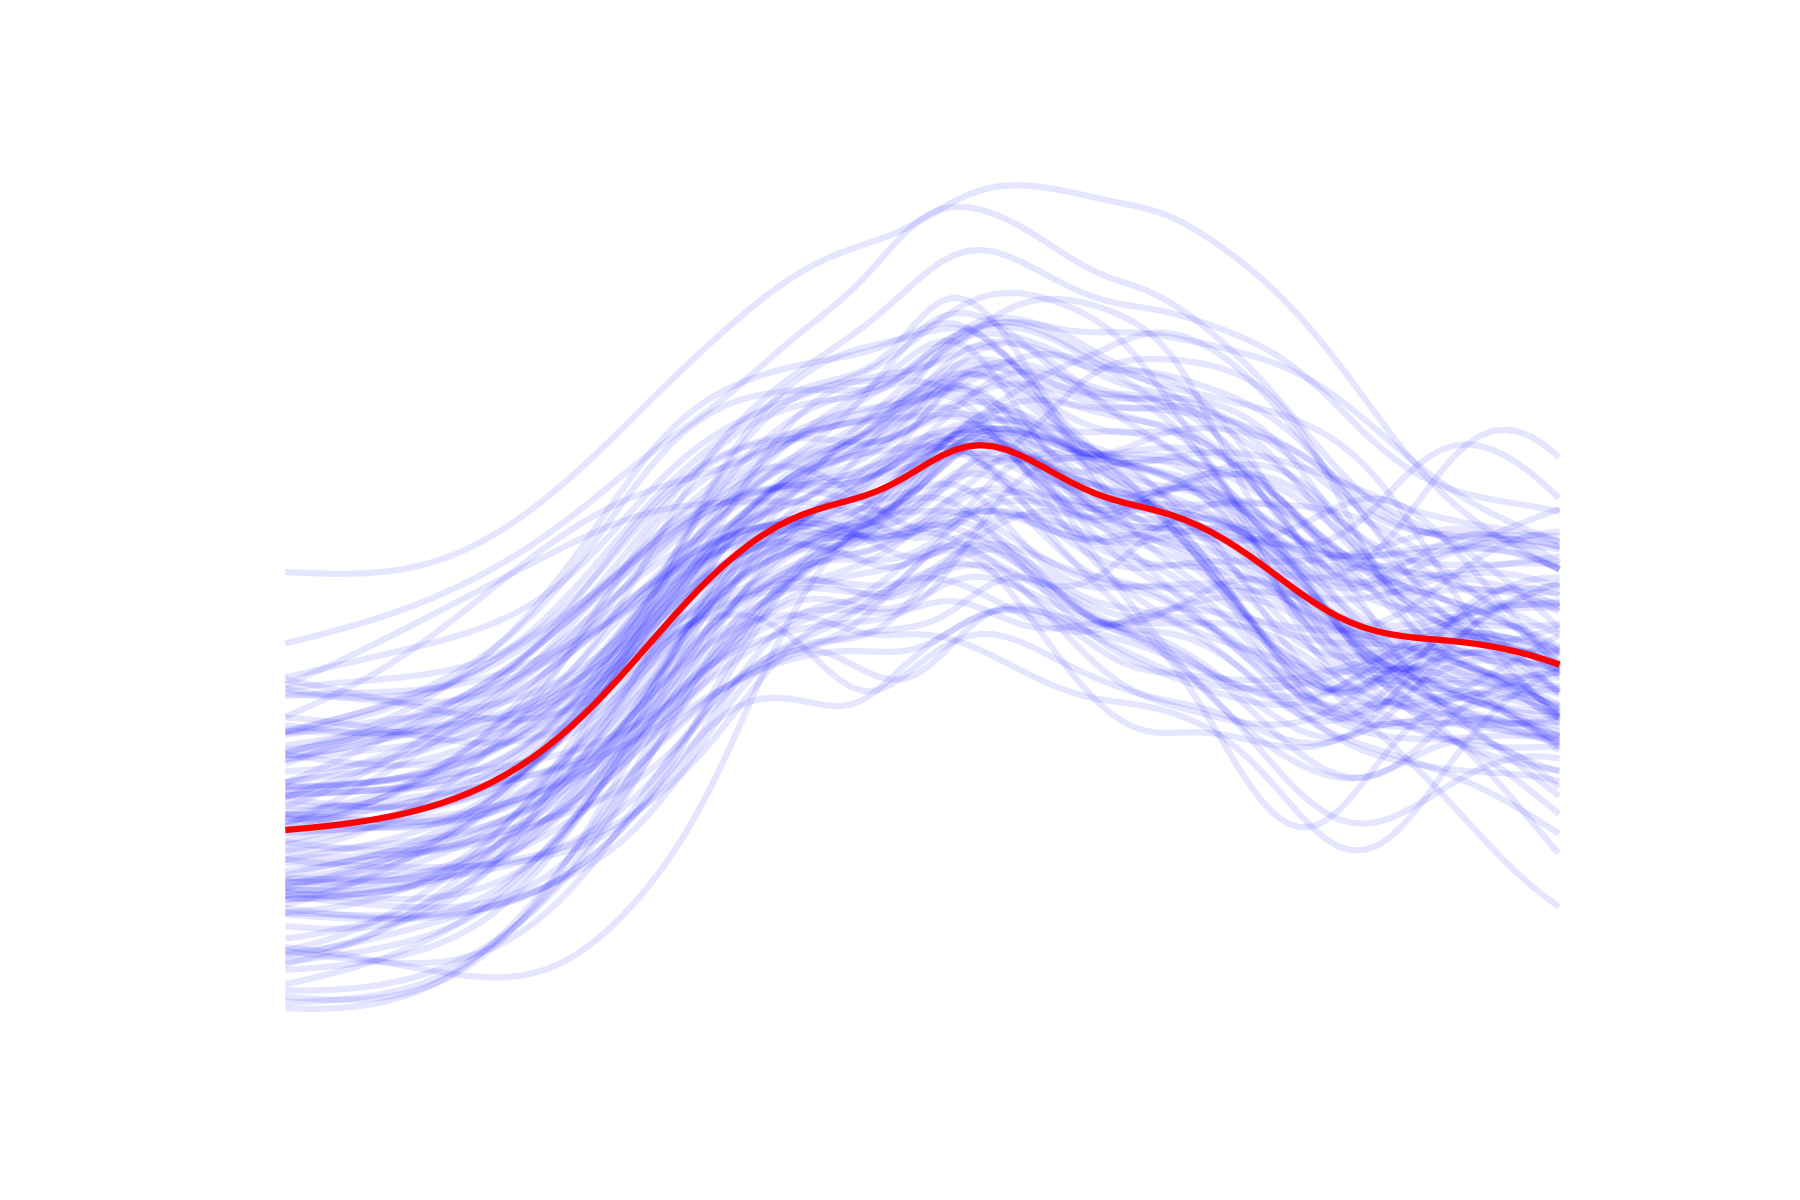
\includegraphics[width=1.8cm]{nonsymnet.png}
};

%%%%%%%%%%%%%%%%%%%%%%%%%%%%%%%%%%%%%%%%%%%%%%
% Right inset
%%%%%%%%%%%%%%%%%%%%%%%%%%%%%%%%%%%%%%%%%%%%%%

\node[
    draw=red!35,
    rounded corners=2pt,
    fill=white,
    inner sep=2pt
]
(PlotR)
at (6.5,1.2)
{
    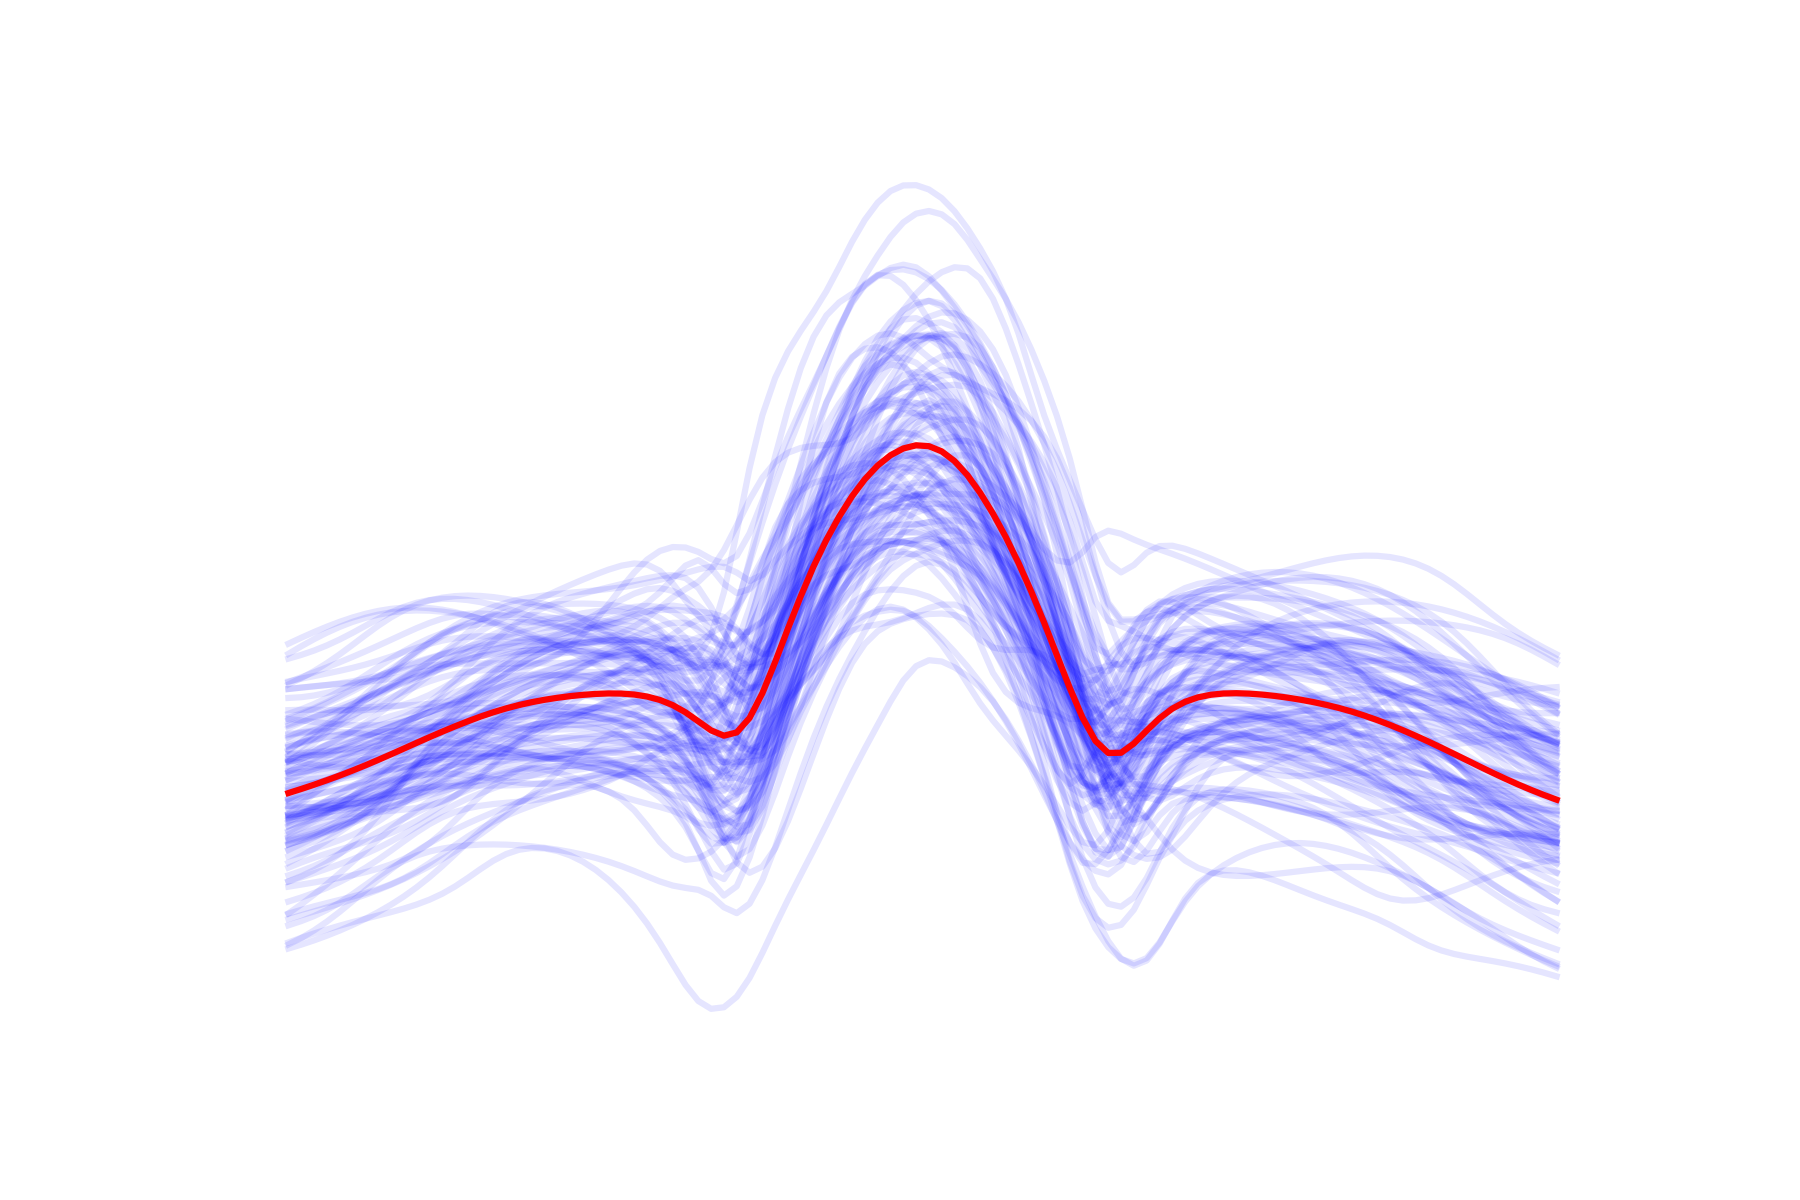
\includegraphics[width=1.8cm]{symnet_spara.png}
};

\draw[black]
    ($(PlotL.center)+(.05,-0.8)$)
    --
    ($(PlotL.center)+(.05,0.8)$);

\draw[black]
    ($(PlotR.center)+(0.02,-0.8)$)
    --
    ($(PlotR.center)+(0.02,0.8)$);

    
\draw[black]
    ($(PlotN.center)+(0,-0.8)$)
    --
    ($(PlotN.center)+(0,0.8)$);

\draw[
     {Latex[length=1mm]}-{Latex[length=1mm]},
    black!60,
    line width=0.4pt,
]
($(PlotL.center)+(-0.35,0.65)$)
arc[start angle=180,end angle=0,radius=0.35];

\draw[
     {Latex[length=1mm]}-{Latex[length=1mm]},
    black!60,
    line width=0.5pt,
]
($(PlotR.center)+(-0.35,0.65)$)
arc[start angle=180,end angle=0,radius=0.35];

\draw[
     {Latex[length=1mm]}-{Latex[length=1mm]},
    black!60,
    line width=0.4pt,
]
($(PlotN.center)+(-0.35,0.65)$)
arc[start angle=180,end angle=0,radius=0.35];

\draw[black!50]
    ($(PlotN.center)+(0,-0.8)$)
    --
    ($(PlotN.center)+(0,0.8)$);

\node[
    black,
    font=\scriptsize
]
at ($(PlotN.center)+(0,.99)$)
{$\times$};

%%%%%%%%%%%%%%%%%%%%%%%%%%%%%%%%%%%%%%%%%%%%%%
% Bezier connectors: dots <-> image frames
%%%%%%%%%%%%%%%%%%%%%%%%%%%%%%%%%%%%%%%%%%%%%%

% Non-symmetric dot (top of the down-arrow) -> west of top frame
\draw[
    gray!60,
    dotted,
    line width=0.7pt
]
(N) --
% .. controls (-3.2,3.7) and (-2.9,3.4) ..
(PlotN.west);

% East of left symmetric frame -> beginning of the thick red line (S1)
\draw[
    red!55!black,
    dotted,
    line width=0.7pt
]
(PlotL.east)
.. controls (-3.7,0.9) and (-5.1,-0.5) ..
(S1);

% End of the thick red line (S2) -> west of right symmetric frame
\draw[
    red!55!black,
    dotted,
    line width=0.7pt
]
(S2)
.. controls (4.7,-0.8) and (4.0,0.5) ..
(PlotR.west);

\end{tikzpicture}